\documentclass[11pt]{article}
\usepackage{acl2014}
\usepackage{times}
\usepackage{url}
\usepackage{latexsym}
\usepackage{graphicx}
\usepackage{hyperref}
\title{Survey on Traffic Flow prediction}

\author{Bingyu Shen \\
  Student ID: 5130309283\\
    {\tt sby2013@sjtu.edu.cn}
}

\date{}

\begin{document}
\maketitle
\begin{abstract}
  This document is a short survey for short term traffic flow prediction approaches. There are several kinds of approaches so far. 1) Time series approaches 2) probabilitstic graphs 3) nonparametric techniques 4) kalman filter. I will list related papers and compare the classic approaches in this article.
\end{abstract}

\section{Introduction}
Why traffic flow prediction?
\begin{enumerate}
	\item Better traffic modeling for intelligent traffic system(ITS).
	\item Better traffic management to avoid congestion and accident.
\end{enumerate}

Traffic flow prediciton is the critical problem in ITS.
\section{Task of traffic flow prediction}
$X_i^t$ is the observed traffic flow quantity at the $i_{th}$ observation location at time interval $t$.
\begin{enumerate}
	\item \textbf{Input:} Observed traffic flow sequence at $i_{th}$ loaction, $\{X_i^t\}$ , which $t \in \{1,2,\dots, T\} $.
	
	\item \textbf{Output:} Traffic flow at given time $X_i^{t+\Delta}$, which $\Delta$ is the time prediction horizon . 
\end{enumerate}


\section{Approaches}
\subsection{Time series}
Time series approaches aims to finding patterns of the temporal variation of traffic flow and then use that information for prediction. Of all these kind of models, (Autoregressive integrated moving average)ARIMA model is mostly used and often used to compare with.

\begin{enumerate}
	\item Bayesian time series model for short-term traffic flow forecasting, 2007
	\item Short term traffic forecasting using time series methods, 1998
	\item Predictions of urban volumes in single time series, 2010
	\item Combining Kohonen maps with ARIMA time series models to forecast traffic flow, 1996 
\end{enumerate}

The time series analysis method are implemented in a library of python - 
\href{http://www.statsmodels.org/stable/index.html}{\tt{Statsmodels}}

\begin{itemize}
	\item \textbf{Advantages:} Each step has clear meaning; mature statical analysis method.
	
	\item \textbf{Disadvantages:} 1) often need linear architecture 2) has a delay of prediction as the results, which can be seen as a lag of prediction based on the historical data. As shown in Figure 1, there is a typical lag in the prediction. 3) Show relatively bad results compared to Deep Learning methods in recent papers.
\end{itemize}
\begin{figure}[ht]
	\centering
	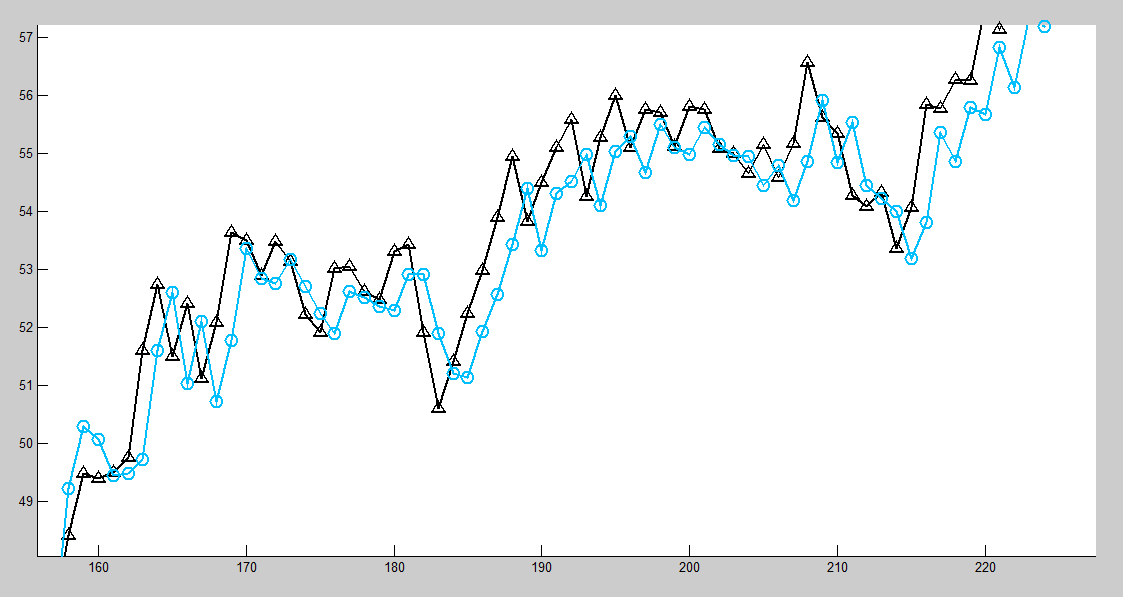
\includegraphics[width=2.5in]{pic1.png}
	\caption{Time series ARMA prediction}
\end{figure}
\subsection{Probabilistic graph approaches}
This method look at the problem from a probabilistic graph persepective, such as Markov chain, Markov Random Fields and Random fields.  From the  standpoint  of  Bayesian  theory,  the  value  of  an  object node can be inferred by its neighbor nodes. So forecasting the incomplete data is possible.
\begin{enumerate}
	\item Variational inference for the infinite mixtures of Gaussian processes with applications on traffic flow prediction, 2011
	\item A Bayesian network approach to traffic flow forecasting, 2006
	\item Short tern traffic flow forecasting based on Markov chain model, 2003
\end{enumerate}

\begin{itemize}
	\item \textbf{Advantages:} Prediction from probilitistic view and the second paper claims to work when data is incomplete.
	
	\item \textbf{Disadvantages:} 1) Time-consuming, difficult to converge(Gaussian Process) 2) Not thorough experiment in the paper
\end{itemize}

\subsection{Nonparametric techniques} 
Applied to scenarios that data is of high uncertainty and complex nonlinearity. Such as artificial neural networks, support vector regression and local weighed learning.

\begin{enumerate}
	\item Online-SVR for short-term traffic flow prediction under typical and atypical traffic conditions, 2009
	\item Traffic prediction using multivariate nonparametric regression, 2012
	\item An online approach based on locally weighted learning for short-term traffic flow prediction
	\item Short-term traffic flow prediction: Neural Network approach
	\item Deep architecture for traffic flow prediction: Deep belief networks with multitask learning
	\item Traffic flow prediction with big data: A Deep learning approach
\end{enumerate}

\subsection{Kalman Filter}
Dynamic Prediction of Traffic Volume through Kalman Filtering Theory. 
\end{document}
